\documentclass[oneside,a4paper]{book}
%\pagestyle{headings}
% $Author: oscar $
% $Date: 2009-11-06 14:37:12 +0100 (Fri, 06 Nov 2009) $
% $Revision: 29604 $
%=============================================================
% ST80 listings macros
% Adapted from Squeak by Example book
%=============================================================
% If you want >>> appearing as right guillemet, you need these two lines:
%\usepackage[T1]{fontenc}
%\newcommand{\sep}{\mbox{>>}}
% Otherwise use this:
\newcommand{\sep}{\mbox{$\gg$}}
%=============================================================
%:\needlines{N} before code block to force page feed
\usepackage{needspace}
\newcommand{\needlines}[1]{\Needspace{#1\baselineskip}}
%=============================================================
%:Listings package configuration for ST80
\usepackage[english]{babel}
\usepackage{amssymb,textcomp}
\usepackage{listings}
% \usepackage[usenames,dvipsnames]{color}
\usepackage[usenames]{color}
% \definecolor{source}{gray}{0.95}
\lstdefinelanguage{Smalltalk}{
%  morekeywords={self,super,true,false,nil,thisContext}, % This is overkill
  morestring=[d]',
  morecomment=[s]{"}{"},
  alsoletter={\#:},
  escapechar={!},
  literate=
    {BANG}{!}1
    {UNDERSCORE}{\_}1
    {\\st}{Smalltalk}9 % convenience -- in case \st occurs in code
    % {'}{{\textquotesingle}}1 % replaced by upquote=true in \lstset
    {_}{{$\leftarrow$}}1
    {>>>}{{\sep}}1
    {^}{{$\uparrow$}}1
    {~}{{$\sim$}}1
    {-}{{\sf -\hspace{-0.13em}-}}1  % the goal is to make - the same width as +
    {+}{\raisebox{0.08ex}{+}}1		% and to raise + off the baseline to match -
    {-->}{{\quad$\longrightarrow$\quad}}3
	, % Don't forget the comma at the end!
  tabsize=4
}[keywords,comments,strings]

\definecolor{source}{gray}{0.95}

\lstset{language=Smalltalk,
	basicstyle=\sffamily,
	keywordstyle=\color{black}\bfseries,
	% stringstyle=\ttfamily, % Ugly! do we really want this? -- on
	mathescape=true,
	showstringspaces=false,
	keepspaces=true,
	breaklines=true,
	breakautoindent=true,
	backgroundcolor=\color{source},
	lineskip={-1pt}, % Ugly hack
	upquote=true, % straight quote; requires textcomp package
	columns=fullflexible} % no fixed width fonts
% In-line code (literal)
% Normally use this for all in-line code:
\newcommand{\ct}{\lstinline[mathescape=false,backgroundcolor=\color{white},basicstyle={\sffamily\upshape}]}
% In-line code (latex enabled)
% Use this only in special situations where \ct does not work
% (within section headings ...):
\newcommand{\lct}[1]{{\textsf{\textup{#1}}}}
% Code environments
\lstnewenvironment{code}{%
	\lstset{%
		% frame=lines,
		frame=single,
		framerule=0pt,
		mathescape=false
	}
}{}

% Useful to add a matching $ after code containing a $
% \def\ignoredollar#1{}
%=============================================================
 %seems to create a problem with the preamble command needline already defined

%=============================================================================

\usepackage{amsthm}
\usepackage{xspace}
\usepackage{float}
\usepackage{ifthen}
\usepackage{amsbsy}
\usepackage{amssymb}
\usepackage{balance}
\usepackage{booktabs}
\usepackage{graphicx}
\usepackage{rotating}
\usepackage{multirow}
\usepackage{needspace}
\usepackage{microtype}
\usepackage{bold-extra}
\usepackage{geometry}
\usepackage{varioref}
\usepackage{xcolor}
\usepackage{textcomp}
\usepackage{listings}
\usepackage[normalem]{ulem} %emphasize still italic
\usepackage{ucs}

% \usepackage[utf8]{inputenc}
% \usepackage[htt]{hyphenat}
\usepackage{times}
\usepackage{url}
\usepackage{alltt}
\usepackage{amsmath}
\usepackage{xfrac}
\usepackage{subfigure}
\usepackage{appendix}
\usepackage{stmaryrd}   % for the \shortuparrow
\usepackage[utopia]{quotchap}

\usepackage{setspace}
\usepackage[numbers, sort&compress]{natbib}
\usepackage{mdwlist}        % support for better spaced lists
% allows for temporary adjustment of side margins
\usepackage{chngpage}
\usepackage[normalem]{ulem} 

\usepackage{adjustbox}
\usepackage{verbatim}

% constants

\newcounter{qcounter}

% commands
\newcommand{\n}{$\cdot$}
\newcommand{\y}{\checkmark}
\newcommand{\subscript}[1]{$_{\textrm{\footnotesize{#1}}}$}
\newcommand{\superscript}[1]{$^{\textrm{\footnotesize{#1}}}$}
\newcommand{\vertical}[1]{\raisebox{-4em}{\begin{sideways}{#1}\end{sideways}}}

\newboolean{showedits}
\setboolean{showedits}{true} % toggle to show or hide edits
\ifthenelse{\boolean{showedits}}
{
       \newcommand{\ugh}[1]{\textcolor{red}{\uwave{#1}}} % please rephrase
       \newcommand{\ins}[1]{\textcolor{blue}{\uline{#1}}} % please insert
       \newcommand{\del}[1]{\textcolor{red}{\sout{#1}}} % please delete
       \newcommand{\chg}[2]{\textcolor{red}{\sout{#1}}{\ra}\textcolor{blue}{\uline{#2}}} % please change
	\newcommand{\brs}[1]{\textcolor{orange}{\textbf{\textit{BS:}}#1}}
	\newcommand{\todo}[1]{\textcolor{red}{\textbf{\textit{TODO:}}#1}}
	\newcommand{\meta}[1]{\textcolor{blue}{\textbf{\textit{META:}}#1}}
	\newcommand{\idea}[1]{\textcolor{green}{\textbf{\textit{IDEA:}}#1}}
}{
       \newcommand{\ugh}[1]{#1} % please rephrase
       \newcommand{\ins}[1]{#1} % please insert
       \newcommand{\del}[1]{} % please delete
       \newcommand{\chg}[2]{#2}
}


% ============================================================================
% Put edit comments in a really ugly standout display

\usepackage{xcolor}
\usepackage[normalem]{ulem}
\newcommand{\ra}{$\rightarrow$}


% comments \nb{label}{color}{text}
\newboolean{showcomments}
\setboolean{showcomments}{true}
\ifthenelse{\boolean{showcomments}}
    {\newcommand{\nb}[3]{
        {\colorbox{#2}{\bfseries\sffamily\scriptsize\textcolor{white}{#1}}}
        {\textcolor{#2}{\sf\small$\blacktriangleright$\textit{#3}$\blacktriangleleft$}}}
     \newcommand{\version}{\emph{\scriptsize$-$Id$-$}}
%	 \newcommand{\ugh}[1]{\textcolor{red}{\uwave{#1}}} % please rephrase
%	 \newcommand{\ins}[1]{\textcolor{blue}{\uline{#1}}} % please insert
%	 \newcommand{\del}[1]{\textcolor{red}{\sout{#1}}} % please delete
%	 \newcommand{\chg}[2]{\textcolor{red}{\sout{#1}}{\ra}\textcolor{blue}{\uline{#2}}} % please change
	 \newcommand{\chk}[1]{\textcolor{ForestGreen}{#1}} % changed, please check
	}
    {\newcommand{\nb}[3]{}
     \newcommand{\version}{}
	\newcommand{\chk}[1]{} % changed, please check
	}

% ============================================================================
% Make quotes be italic
\renewenvironment{quote}
    {\list{}{\rightmargin\leftmargin}%
     \item\relax\begin{it}}
    {\end{it}\endlist}

\newcommand{\ttimes}{\ensuremath{\times}}

%=============================================================================

%\newcommand{\needlines}[1]{\Needspace{#1\baselineskip}}

% source code
\usepackage{xcolor}
\usepackage{textcomp}
\usepackage{listings}
\definecolor{source}{gray}{0.9}
\lstset{
	language={},
	% characters
	tabsize=3,
	upquote=true,
	escapechar={!},
	keepspaces=true,
	breaklines=false,
	alsoletter={:},
	breakautoindent=true,
	columns=fullflexible,
	showstringspaces=false,
	basicstyle=\footnotesize\ttfamily,
	% background
	frame=single,
    framerule=0pt,
	backgroundcolor=\color{source},
	% numbering
	numbersep=5pt,
	numberstyle=\tiny,
	numberfirstline=true,
	% captioning
	captionpos=b,
	numberbychapter=false,
	% formatting (html)
	moredelim=[is][\textbf]{<b>}{</b>},
	moredelim=[is][\textit]{<i>}{</i>},
	moredelim=[is][\uline]{<u>}{</u>}}
%\newcommand{\ct}{\lstinline[backgroundcolor=\color{white},basicstyle=\footnotesize\ttfamily]}
%\newcommand{\lct}[1]{{\small\tt #1}}


%----------------------------------------------------------------------------
% references
\newcommand{\tabref}[1]{\hyperref[{tab:#1}]{Table~\ref*{tab:#1}}}
\newcommand{\figref}[1]{\hyperref[{fig:#1}]{Figure~\ref*{fig:#1}}}
\newcommand{\secref}[1]{\hyperref[{sec:#1}]{Section~\ref*{sec:#1}}}
\newcommand{\lstref}[1]{\hyperref[{lst:#1}]{Listing~\ref*{lst:#1}}}
\newcommand{\charef}[1]{\hyperref[{cha:#1}]{Chapter~\ref*{cha:#1}}}
%----------------------------------------------------------------------------

% abbreviations
\tracingcolors 4
\setcounter{tocdepth}{3}
\setcounter{secnumdepth}{3}
\newcommand{\ie}{\emph{i.e.,}\xspace}
\newcommand{\eg}{\emph{e.g.,}\xspace}
\newcommand{\etc}{\emph{etc.}\xspace}
\newcommand{\etal}{\emph{et al.}\xspace}


\newcommand{\newevenside}{
	\ifthenelse{\isodd{\thepage}}{\newpage}{
	\newpage
        \phantom{placeholder} % doesn't appear on page
	\thispagestyle{empty} % if want no header/footer
	\newpage
	}
}

\def\stretchfactor{1}
\newcommand{\mychapter}[1]{\setstretch{1}
    \chapter{#1}\setstretch{\stretchfactor}}

%----------------------------------------------------------------------------
\newcommand{\lessSpace}{\vspace{-1em}}
\DeclareGraphicsExtensions{.pdf,.png}
\graphicspath{{images/}}
\newcommand{\fig}[4]{
	\begin{figure}[#1]
		\centering
		\includegraphics[width=#2\textwidth]{#3}
		\lessSpace
		\caption{\label{fig:#3}#4}
	\end{figure}}

% ===========================================================================

%:CONFIGURE THIS

\newcommand{\thesistitle}{TestView Plugin}
\newcommand{\thesisauthor}{Dominic Sina}
\newcommand{\thesisauthorOrigin}{Zollikofen BE, Switzerland}
\newcommand{\thesisleiter}{Prof.\ Dr.\ Oscar Nierstrasz}
\newcommand{\thesisasst}{Boris Spasojevi\'c}
\newcommand{\thesisurl}{http://scg.unibe.ch/}
\newcommand{\thesissubtitle}{A Nautilus Plugin to facilitate Unit Testing}
\newcommand{\thesisdate}{05. Februar 2015}

% ===========================================================================

\usepackage[ colorlinks=true, urlcolor=black, linkcolor=black,
			citecolor=black, bookmarksnumbered=true, bookmarks=true,
			plainpages=false,
			pdftitle={\thesistitle}, pdfauthor={\thesisauthor},
			pdfsubject={\thesissubtitle}, pdfpagelabels]{hyperref}

\newcommand{\hrref}[2]{\hyperref}
% ===========================================================================
% ===========================================================================


% D O C U M E N T
% % % % % % % % % % % % % % % % % % % % % % % % % % % % % % % % % %
\begin{document}

% T I T L E
% % % % % % % % % % % % % % % % % % % % % % % % % % % % % % % % % %
\begin{titlepage}  
  \begin{center}  
  
  \begin{figure}[t]  
  \vspace*{-2cm}        % to move header logo at the top 
  \center{
\includegraphics[scale=0.5]{logos/UNI_Bern.png}}
  \vspace{1.2in}     
  \end{figure}

    \thispagestyle{empty}
    
    {\bfseries\Huge \thesistitle \par
    \Large \vspace{0.1in} \thesissubtitle \par}

    \vspace{0.3in} 
    \LARGE{\textbf{Bachelor Thesis} \\}
    \vspace{0.4in}

    {\Large \thesisauthor \par from \par \thesisauthorOrigin}
    
    \vspace{0.3in}
    {\Large Philosophisch-naturwissenschaftlichen Fakult\"{a}t \\
            der Universit\"{a}t Bern \par}
    \vspace{0.3in}
    {\Large \thesisdate \par}
    \vspace{0.3in}
    %Leiter der Arbeit: \par
   {\Large \thesisleiter} \par
      {\Large \thesisasst} \par
   \vspace{0.1in}
    {\Large Software Composition Group \par Institut f\"{u}r Informatik und angewandte Mathematik \par University of Bern, Switzerland \par}
  

  %\vspace{0.5in}
 
 

  \end{center}

\end{titlepage}


% A B S T R A C T
% % % % % % % % % % % % % % % % % % % % % % % % % % % % % % % % % %
\chapter*{\centering Abstract}
	\begin{quotation}
		\noindent 
\meta{content:unit test friendly environment, nautilus plugin, introduce main functionalities}
The purpose of this bachelor project is to improve the Pharo environment by making it more unit test friendly. Instead of writing a new system browser we chose to realize this as a Nautilus plug-in since this makes it easy to set up and builds on established parts of the Pharo environment. This plug-in includes various functionalities that help with finding and writing unit tests. 
Further it provides ways to check if a method is untested, to see all tests that have been written for a certain method, to add new tests to existing methods and the ability to view a method and a corresponding test side by side. 
Before explaining the plug-in and its functionalities in more detail we will take a look at various terms surrounding unit testing and analyze the develop environments Eclipse and Pharo. They will be compared to each other in how unit test friendly they are and opportunities to improve them will be discussed. The aim of this thesis is to take a closer look at unit testing and in form of a Nautilus plug-in provide an example of how unit testing can be facilitated. 

\idea{more focused on improved UI and everything resulting from this. Other directions to improve unit test friendlyness would be hierarchical tests amongst other things.}

\idea{The user can then add and remove elements from the resulting collection of tests to ensure that only actual tests are shown. These features not only facilitate unit testing but can also be used to help understanding methods by looking at their tests.(too much detail for there?) }
	\end{quotation}
\clearpage


% C O N T E N T S 
% % % % % % % % % % % % % % % % % % % % % % % % % % % % % % % % % % % % % % % %
\tableofcontents

%%%%%%%%%%%%%%%%%%%%%%%%%%%%%%%%%%
%%%% Introduction %%%%%%%%%%%%%%%%%%%%%
%%%%%%%%%%%%%%%%%%%%%%%%%%%%%%%%%%
\chapter{Introduction}
	\label{cha:introduction}
\meta{testing => benefits of testing by itself => Current development methods => break the cycle of frustration}
Testing has become a very important part of software development. The reason for this is that testing is useful to validate a project. While it is true that ``[p]rogram testing can be used to show the presence of bugs, but never to show their absence!'' \cite[p.~6]{Dijk72b} testing still helps to validate at least parts of the functionality of a program. Tests are for example useful to determine if newly written code behaves as expected and can also be used to detect if recent changes break previously working code (regression errors).
 
User studies indicate that about 10-15\% of the development time is spend waiting for tests to finish executing and fixing regression errors, and simply increasing the frequency with which the tests are performed reduces this wasted time by 31-81\% \cite[p.~1]{Saff03b}. This also means that the additional time it takes to execute tests more frequently is less than the time saved by fixing regression errors early.

Since testing provides these benefits it has become a key feature of many current software engineering paradigms like for example extreme programing (XP) \cite[p.~1]{Pres14a}. Together with the other features of these development methods testing helps to speed up the development and increase the quality of the software being developed. Additionally for example in XP the time that is spent writing a test will be regained. As Wells\cite{Well13a} puts it: ``...during the life of a project an automated test can save you a hundred times the cost to create it... ''. This is done by guarding against bugs and regression errors. Since this guard is in place "refactoring" and "frequent integration" of new code become possible. 

This brings us the problem that while testing clearly has its benefits it is still seen as optional or too time consuming by many. That many developers underestimate the difference that unit tests can make becomes evident in that even when there are tests they are not executed as often as they should be. In their case studies Pressman and Ernst found that the 31-82\%  reduction of waisted time can be achieved by simply running the same tests two to five times as often\cite[p.~1]{Pres14a}. The reason why the effect of testing is underestimated is that often under stress the more direct and optimistic way of implementing more features instead of testing seems faster. This will in the long run slow down the development process since all the previously discussed benefits of testing are missing. So there might be no time for testing in the future as well. 

Breaking out of this circle can require an outside influence \cite{Beck98a}. While certainly some developers have no problem writing tests no matter the situation a little encouragement might be need for others. In this bachelor thesis we attempt to provide another one of those outside influences by making testing easier and faster.

\chapter{A Closer Look at Testing}
	\label{cha:Testing}
\meta{content:define terminology of testing paradigms} 
\brs{on first look, this is not much of an introduction, this could be a chapter called ``technical background'' or something. The introduction should introduce the reader to the problem in some detail and give short overview of the proposed solution.} In this chapter we will take a look at different testing paradigms in order to specify how these terms are used throughout this thesis. During the next chapters these terms will then be applied to better describe how current programming environments support these paradigms and where precisely this support is lacking. It is important to note that these paradigms are not mutually exclusive. 


\section{Unit Testing}
	\label{sec:Unit Testing}
\todo{automated test vs manualy tests in active development}
\meta{content:unit testing, definition of scope, independant tests}
Unit testing follows the paradigm of isolating the smallest inseparable parts of a program and testing them independently of each other. Each of these tests is done as low level as possible. System wide tests are generally not a part of unit testing. 
This means that the scope of each test is very small and consequently many tests are needed to cover \chg{a}{the} whole implementation. By making unit tests one ensures that the tested method behave as expected.\rm{and also speeds up development since these automated test are very fast to execute.} \brs{writing tests speeds up development(not true) because tests are fast to execute(makes no sense)} 

\meta{u.t. in smalltalk->methods->preconditions, mocks->postconditions after method invoc, mocks}
In Smalltalk these smallest units are often methods since the language heavily relies on sending messages (what roughly translates to a method invocation in other languages) between objects. 
To start testing an instance of the object providing the method under test is created and brought into a state where a set of preconditions is met. An example for preconditions would be the requirement for the objects instance variables to have certain values. From this initial state in a deterministic environment a specific outcome can be expected after the method is executed. The outcome is a success if all of the previously defined postconditions are fulfilled.

To illustrate this let us examine how unit tests for a simple stack might work. The stack has a maximum capacity that is set once the stack is created. Further the stack provides a method named "push(x)" which adds an element "x" on top of the stack and  a method named "pop()" which removes and returns the element that was added last to the stack. Now let us examine how to make a unit test for this stack that checks if the last element that was added is returned by "pop()" and not some other object. The preconditions need to make sure that the stack is initialized with a capacity bigger than zero. If no stack is created or if its size is smaller than one then the stack can return nothing even if everything is correctly implemented. After this precondition the test will now call "push(x)" and then "pop()". Now we need to make sure that operations work as expected or in other word we need to check our postconditions. In this case if the object returned by "pop()" is the one that we pushed to the stack and that the stack is empty again after the element was popped.

%\idea{remove this section mocks are not important in this paper}
%To simplify the setup of those preconditions and to keep the tests independent mock objects are often used to emulate the behavior of other objects besides the \chg{object}{class} containing the tested method \brs{classes contain methods, not objects}. That way \del{it can be avoided} having to fully prepare these other objects \ins{can be avoided} and since these mocks do not execute the real code faults in the mocked objects do not impact other tests.

\meta{summary of previous paragraphs}
For the purpose of this paper two features of unit testing are important to keep in mind. The first one is that unit testing takes place at a method level and the second one is that the narrow scope of unit tests requires many tests to cover multiple methods. Further\ins{,} due to how it is recommended to keep each test as small as possible even a single method is likely to require multiple corresponding tests since every path in the decision tree of the method should be covered.

\section{Test-driven Development}
	\label{sec:Test-driven Development}
\meta{ttd is concerned with the order of implemetation}
In Test-driven Development the tests for a \chg{application}{functionality} are written slightly before the \chg{application}{functionality} itself. Afterwards the \chg{application}{functionality} is implemented until those tests are satisfied. After this more tests are added to test additional functionality. This process is repeated until the feature is working. Test-driven development thus requires the developers to regularly determine the requirements for a functionality.
A comprehensive overview of the most important rules in Test-driven Development can be found here \cite[p.~122]{Mart09a}:
\begin{quote}
First Law: You may not write production code until you have written a failing unit test.

Second Law: You many not write a more of a unit test than is sufficient to fail, and not compiling is failing.

Third Law: You may not write more production code than is sufficient to pass the currently failing test.
\end{quote}
While it might seem tedious this repeated careful planning is \del{also} the biggest advantage of this approach. Applications developed with Test-driven Development have to be very thought-out and every requirement has to be clear since those are required to begin writing the the production code.

\meta{facilitating unit testing in ttd is different since no data can be gathered from the implemented method at first}
As shown in \autoref{sec:Unit Testing} it is fair to look at testing on a method level when discussing unit testing. Since in Test-driven Development the methods may not have been written when the test\ins{s} are created the method declarations and the method locations in the class hierarchy can not always be used to make certain assumptions that could be used to facilitate creating new tests. For example before a method in the production code is written it needs to have a failing tests that checks if this method exists. Only for subsequent tests to the same method can the method declaration and the method location in the class hierarchy be found in the production code.

Test-driven Development bears mentioning because it is one of the major paradigms concerned with testing and because in the context of this paper it has to be treated a bit differently. Namely since it is not possible to always get the method declaration and location in the class hierarchy to help generating tests when doing Test-driven Development.

\section{Blackbox and Whitebox Testing}
	\label{sec:Blackbox and Whitebox Testing}
\meta{whitebox=aware of inner workings, blackbox=unaware}
Whitebox and blackbox testing refer to how closely tests are written to suit a method. In whitebox testing the tester is completely aware of the method and its inner workings when writing a test for it. This means that an adequate amount of unit tests done with a whitebox approach will cover each important path in the decision tree of a method. Especially interesting are worst case scenarios that can be found by examining the code and method invocations that result in as much executed lines as possible.

Contrary in blackbox testing the test writer does not know the inner workings of the method that is being tested. Ghezzi et al. describe that during blackbox testing "[t]est sets are developed and their results evaluated solely on the basis of the specifications" \cite[p.~282]{Ghez02a}. This means that the tests have to be made so that they return the right value for all tested input values. Since it might be unfeasible to test all values it is necessary to choose the critical input values where an error might occur.

\meta{what should be remembered}
For the purpose of this paper it is important to remember that depending on which one of those paradigms is used it is necessary to have in depth knowledge of the method being tested in order to write a test for it. Namely while doing whitebox testing. On the other hand when doing blackbox testing it is discouraged to look at the implemented method, provided it has already been written.

%\section{The Nautilus Plugin Framework}
	%\label{sec:The Nautilus Plugin Framework}
%TODO, or leave it out? probably yes, I have enough to write about

%%%%%%%%%%%%%%%%%%%%%%%%%%%%%%%%%%
%%%% The Problem %%%%%%%%%%%%%%%%%%%%%
%%%%%%%%%%%%%%%%%%%%%%%%%%%%%%%%%%
\chapter{The Problem}
	\label{cha:The Problem}
\meta{Important features: 
has tests?
show all tests to a method
helps adding new tests with templates, packages and clases
view test and method at the same time}

\meta{missing features for easy unit testing, list needed features, why are they important based on testing paradigms}
As shown in \autoref{cha:introduction} many current software development paradigms rely on unit testing but as important as unit testing is not all current development environments are optimized for it. For example the search for unit tests to a specific method is often lacking or not present at all. 
In this work we assume that important features for unit test friendly environments are a quick way to see if a method is tested, an automated test search, the ability to view tests and methods side by side and an option to easily create new tests. These criteria are based on the definitions of the various testing paradigms previously described in \autoref{cha:Testing}. 

Namely unit testing can be supported by letting the developer see if a method is covered by at least one test, the search for all tests corresponding to a specific method and the ability to create new tests as fast as possible. 
In whitebox testing it is convenient to see the method under test and the test at the same time without switching between the two. With this it becomes easier to write tests that together cover each path in the decision tree of the method.

Since not many environments were created with specifically unit testing in mind there are often some of these features missing. Concrete examples of environments lacking these specific features will be pointed out in \autoref{cha:Related Work}. To compensate for this the user is required to manually execute many tasks like navigating back and forth between method and test and creating new test classes and packages. This repeatedly breaks the programmers flow and in effect discourages them from writing tests. In the following we will take a closer look at the tasks involved in different goals which will help to understand the problem of those missing functionalities and exactly at which point they are needed.

\section{Is a method tested?}
\label{sec:Is a method tested?}
\meta{check if a method is covered by a test}
In unit testing it is important that each method is tested. As discussed in \autoref{sec:Unit Testing} a method with no tests is unsafe and might even have to be tested manually which is quite slow. Thus a very important feature in unit testing is the ability to check if a method has at least one test. This has to be as easy to see and as uninterruptive as possible. 

If this feature is not implemented the user has to switch back and forth between a class and all its test classes to check manually. If the test classes are not known to them they have to find them first. Both of those tasks can take a lot of effort. 
Luckily code coverage tools also provide this functionality. They allow \del{letting} the user \ins{to} run test suits and then see which part of the implementation were executed. This \ins{will} \del{will} \chg{tell}{show} if a method never got called \del{when running a certain test suit} and \chg{this}{thus} is untested.

\section{Showing all tests to a method}
\label{sec:Showing all tests to a method}
\meta{see all tests to a method, combine with functionality above}
Resulting from unit testing is the requirement to look up a method and all the tests that have been written for it. Just checking if a method is tested at all is not enough, the user wants to see if the method is tested sufficiently. To ensure this multiple test methods are required. Also If at least one test for a method could be found then the method is not untested. This functionality can thus easily substitute the one described in \autoref{sec:Is a method tested?}. The previous ability to see if a method is untested will thus no longer be discussed separately in this paper. 

Similar to showing if a method is tested this helps the user to decide if it is necessary to write a new test. Additionally this functionality helps the user see if a certain test case has already been created and thus is not need again. Further a user could study how a method works by looking at the corresponding tests. 

A lack of this test search function will require great effort on part of the user to keep track of  test classes and test methods. If the user decides to add a new test then it is necessary to take a short look at every test to determine if a similar test has not been written. In this case the tester needs to have quick access to all tests of this method. A lack of this feature makes unit testing in anything but the smallest applications very tedious and new testers will have trouble getting an overview of the existing test suit.

Since this test search relies strongly on the relation between tests and method code coverage tools provide less help. 
To be useful the code coverage tool would have to save for each method from which test it was called during the execution of a test suit. Also coverage is not necessary a good metric to determine if a tests actually tests a method. Nested method calls might yield a large number of false positives. 

\brs{thus far much talk about a lot of important stuff, not enough about what \emph{exactly} the problem is and why}
\dos{did breaking it up into sections work?}

\section{Creating new tests}
\label{sec:Creating new tests}
\meta{facilitate the creation of new tests}
As discussed previously it should be as simple as possible to check if a method is not sufficiently tested. Almost as a direct consequence the user has to create these new tests if this is the case. Especially at the start of a project many new tests will have to be created. So it is safe to say that in unit testing another reoccurring user goal is the creation of new tests for methods with no or too \chg{less}{few} tests.

While creating a new test the user first has to decide in which package and class the new test will be added. In many cases the location of this new test has already been decided on since other tests corresponding to the same method are already there. In this case a quick option to specify an existing test class should be offered. If there are no test classes and packages or if the existing ones do not fit the new test then the user has to create new ones. 

In this case the test package name and the test class name are often derived from the original package and class names. Both of those derivations should be set as default values for the new class and package to possibly save some time. A slight drawback of the derivation of these default names is that the method that is being tested has to be defined previously. Especially when using Test-driven Development the programming environment can not always make such name derivations. During Test-Driven Development only after the first test that verifies if a method is declared has been satisfied these derivations can be made. Provided that tests to the same class will not go into different test classes these default values will not help the user.

As shown it does not matter if the test class and package already exist or if they need to be added. Either way it is possible to support the user during the creation of a new test except during the creation of the first test to a method in Test-Driven development. The creation of new tests can be facilitated by providing a fast way to specify an existing test class and giving default names for new test classes and packages. 

While it helps to have these aids a lack of them seems not as bad as a lack of the test search functionalitiy described previously in \autoref{sec:Showing all tests to a method}.

%%%%%%%%%%%%%%%%%%%%%%%%%%
\todo{continue correcting here}
%%%%%%%%%%%%%%%%%%%continue making this into a section and proofreading it
\meta{see method and test side by side}
Resulting from whitebox testing is the need know a method's inner workings while testing. It is expected that the programmer who writes the test is trying to test every line of code. Thus it is important to provide the user with information on how the method works. Ways to do this include writing notes or showing selected sections of the tested method but the possibly simplest way is to let the users see the whole method in question at the same time as they are writing the test for it. 
In Black-box Testing this feature can be counterproductive. If not desired the additional information can spoil blackbox testing and even if completely ignored it still takes up space on the screen. Blackbox testing thus requires that this feature can be turned off. While this feature is not very important in blackbox testing it helps during whitebox testing. 
Due to the simplicity and effectiveness of the  solution we will focus on letting the user see the method under test and the test that is being written at the same time. It is important not only to provide this functionality but also to optimize it. 
If no information about a method is provided by the programming environment the users have to make notes for themselves, look things up in design documents or resort to additional analysis tools. This can be very tedious and take a lot of time. By making it unnecessary to switch between gathering information about a method, writing tests for it and looking up the same information again a great deal of repetitive manual tasks that the user has to execute becomes obsolete.

\meta{use the discussed functionalities to help analyzing existing environments}
These basic features that a unit test friendly environment should have will be used in the next chapter as a starting point to critically analyze existing environments. If some of these are missing then the user often might have to do simple but also quite repetitive tasks to compensate. This increases the time and effort needed to create unit tests and thus make writing tests a chore. By automating those minor tasks on the other hand various use cases involving unit tests can be simplified. In turn the user is encouraged to write tests what will hopefully increase the quality of the software that is being written.

%%%%%%%%%%%%%%%%%%%%%%%%%%%%%%%%%%
%%%% Related work %%%%%%%%%%%%%%%%%%%%%
%%%%%%%%%%%%%%%%%%%%%%%%%%%%%%%%%%
\chapter{Related Work}
	\label{cha:Related Work}
%view test and method side by side
%ability to find all tests to a certain method
%facilitating adding of tests

\section{\brs{new section}}
%take a look at existing environments
In this section current programming environments, namely Eclipse and Pharo, are analyzed in how unit test friendly they are. Special focus will be placed on the features described in \autoref{cha:The Problem}. These features are: viewing test and method side by side, search all tests to a specified method and facilitating the creation of new tests. The two environments will be compared and possible places for improvement will be discussed.

%eclipse
We will start by taking a closer look at Eclipse since its use is very widespread and it has many parallels to other programming environments like for example Visual Studio. In the picture below\brs{all pictures must me labeled and referred to with the labels} you see a Java project opened in Eclipse with a package and two classes.

\brs{remove the start bar from the pictures}
\begin{figure}[h!]
	\centering
	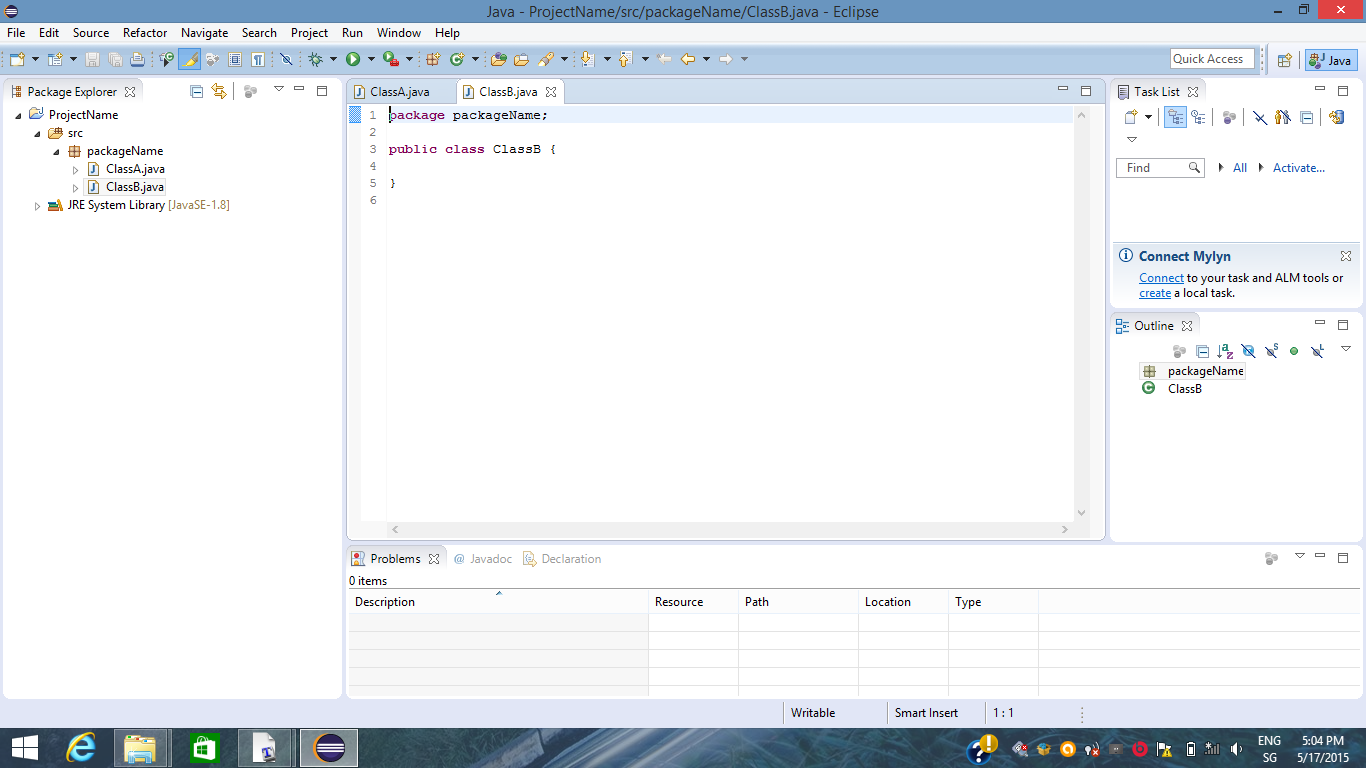
\includegraphics[scale=0.4]{screenshots/eclipseIntro.png}
	\caption{Eclipse's user interface}
\end{figure}

\subsection{\brs{new section}}
\meta{view method and test side by side with tabs}
Let us start with the discussion of how the users can see the tests that they are currently writing and the methods that are being tested at the same time in Eclipse. On the left hand side of the window you can see the Package Explorer. In this file hierarchy you can see every project, package and class. Classes that are opened through the Package Explorer \ugh{or otherwise will then be shown in the middle of the screen and a new tab on top of the code editor will appear}. Unless you close these tabs all the classes you opened \del{last} will be quickly available through their tabs. \del{This is similar to how many Internet browsers work and is easily understood by most through this resemblance.} 
A big advantage of this system is that users can create favorites by not closing important tabs. Through this they can switch back and forth between methods when creating tests. A slight drawback is that the user has to close unneeded tabs from time to time. In most cases the use of these tabs will be smooth enough to allow the programmer to switch uninterrupted between tests and methods via their classes. If for some reason this does not suffice then it is also possible to split the code editor multiple times either horizontally or vertically like on the picture below.

\begin{figure}[h!]
	\centering
	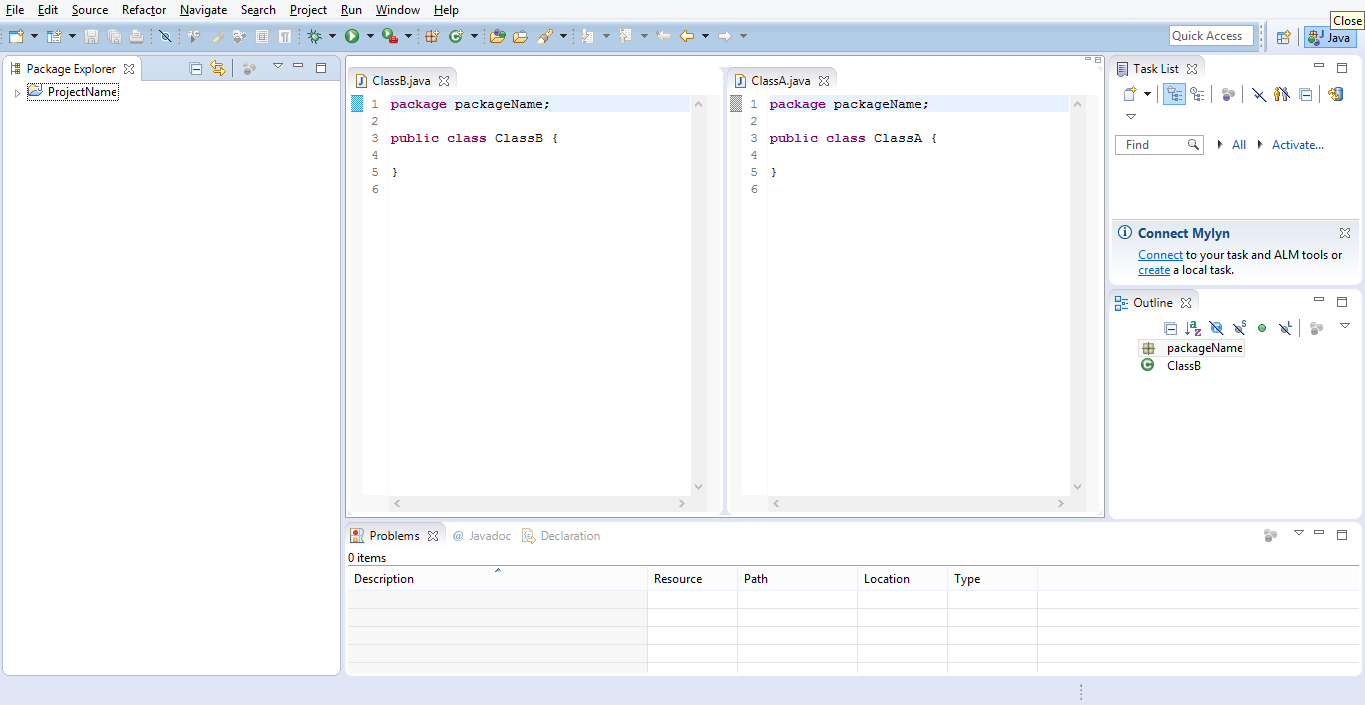
\includegraphics[scale=0.4]{screenshots/eclipseSplitscreen.png}
	\caption{Viewing two classes at the same time}
\end{figure}

As shown Eclipse provides multiple ways to make information about the tested method easily accessible during testing. 

\meta{check if method is untested not present, help with code coverage tools}
\section{\brs{new section}}
Another feature we discussed in the previous chapter was the ability to find all tests to a certain method. In Eclipse this functionality is not included but something similar can be added through various test coverage plugins. As mentioned a code coverage tool can provide a similar functionality. An example of a code coverage plugin for Eclipse is EclEmma. When run on a class containing unit tests the coverage of these tests will be computed. With this it is possible to see if a specific method \ins{is/was} never \del{was} executed while the tests were running and thus is untested. 
Disadvantages of this are that in the test the method under question does not have to be called directly. This can lead to tests covering methods they are not intended to. It also is difficult to tell how many tests for a method have been written depending on how much information the code coverage tool gathers and displays. So while code coverage tools can help managing unit tests its use is limited. In the end a convenient way to find all tests to a given method is missing in Eclipse.

\begin{figure}[h!]
	\centering
	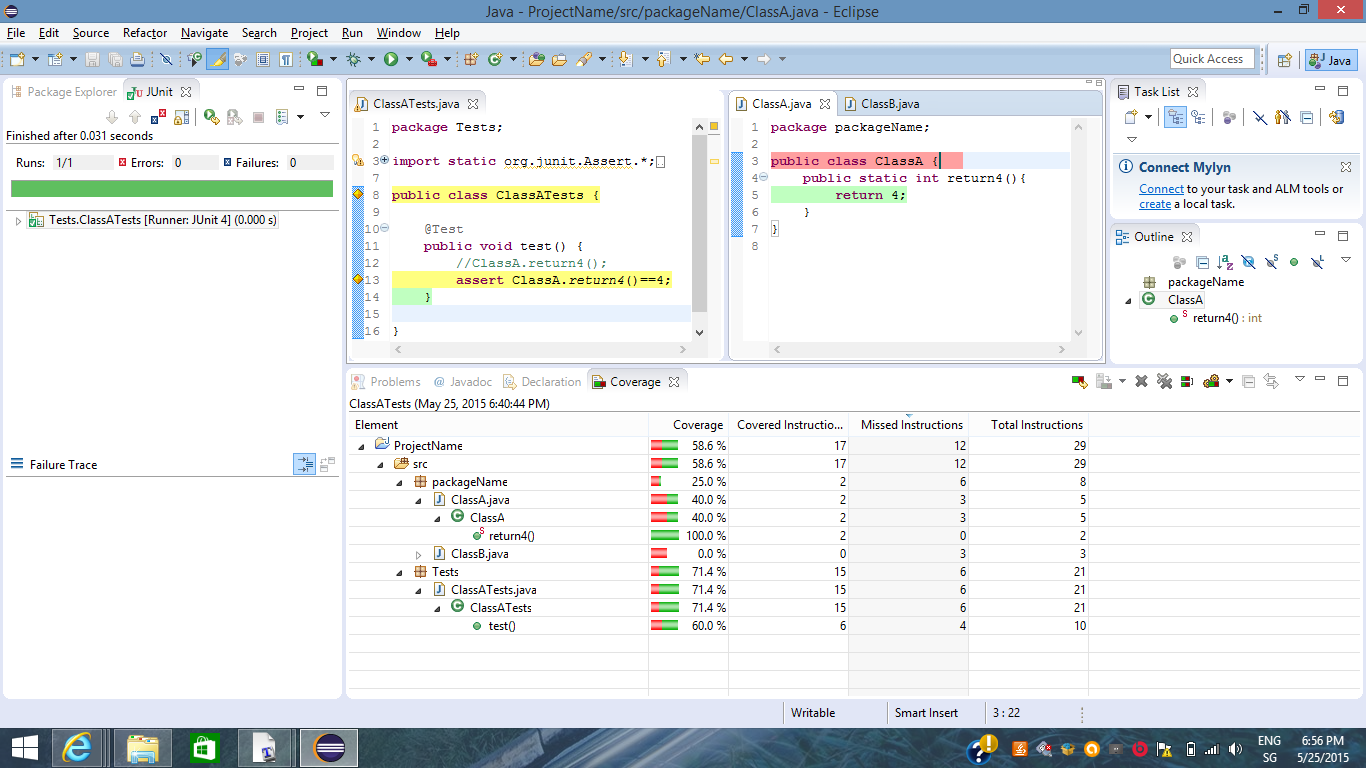
\includegraphics[scale=0.4]{screenshots/EclipseMclEmma.png}
	\caption{MclEmma plugin}
\end{figure}

\subsection{\brs{new section}}
\meta{creating new tests}
\idea{talk more directly about JUnit?}
The next feature in Eclipse we now discuss is how the creation of new tests is facilitated. Eclipse has the option to add a new test class by right clicking on the class that will be tested, selecting "New" from the list that is shown and then clicking "JUnit Test Case". There are other ways to do this but by making sure that the right class is selected in the Package Explorer Eclipse is able to better support the user. In the newly open wizard a default name is already created and the selected class is put into the "Class under test" field. As default package the package of the class under test is used but it can be changed. In this wizard are also other options to create method stubs for standard methods used in JUnit tests which might be useful for the new tests. By clicking on the "Next" button it is possible to select each method of the class under test and appropriate test stubs. 
On one hand this is very good for creating new test classes but on the other hand Eclipse does not provide a way to add new test method\ins{s} \del{stubs} in an already existing test class. Another problem is that through the wizard it is not possible to create more than one test per method in the class under test. Eclipse makes it easy for the user to create new test classes with multiple tests but the creation of new tests in existing classes is only facilitated if it is done one by one.

\subsection{\brs{new section}}
\meta{eclipses strengths and weaknesses, recap}
Although Eclipse is not absolutely optimized for unit testing it is very well sufficient. Eclipse's biggest strengths are the ability to keep recently opened methods as tabs as well as splitting the code editor horizontally and vertically. This is very good for keeping details about a method's implementation close to the user and thus supports whitebox testing. The biggest drawback is the lack of a test search functionality.

\section{\brs{new section}}
%pharo
\meta{pharo}
Now let us take a look at how Pharo and its system browser Nautilus compare to this. It is worth mentioning that \chg{Pharo}{the Pharo IDE} \brs{try to make a clear distinction between Pharo and it's IDE, for clarity} is quite different from Eclipse in that the placement of its visual elements is less rigid. The users are able to customize the appearance of the environment very quickly and adapt it to their wishes. On the other hand Pharo is less wide spread and not as well supported in many ways. 

\subsection{\brs{new section}}
\meta{view test and method side by side, multiple nautilus windows, lock methods}
As with Eclipse the first functionality we will look at is the ability to view tests and methods side by side. Pharo provides a very customizable environment and it is almost necessary for a user to arrange all windows that are created in a way that is comfortable. It is possible to create multiple Nautilus windows and arrange them so that in one the method and in the other the test for this method is shown. Through this a very similar effect to Eclipse's split code editor is achieved. 
The free placement of those Nautilus windows gives the user more freedom to customize the environment but several visual elements will be duplicated which reduces the available space on the screen to arrange these. An example for such a duplicated element is the file hierarchy on the left hand side of each Nautilus window. 
There also exists the option to lock a method and then select a different one inside the same Nautilus window without opening a new one. The users can then see both methods at the same time in the code editor or each individually depending on what they choose. At the moment though there exist problems with this locking mechanism which can lead to multiple code editors being displayed over each other. This makes the method lock function hard to use. 
Apart from this Nautilus also has a History Navigator which allows fast access to all recently viewed methods and classes. This can be used to switch between method and test in way that is comparable to Eclipse's tabs of recently opened classes. The drawback here is that only a certain amount of those recently accessed classes and methods is stored and if the user looks at different methods and classes it is quickly necessary to reopen the previous tests and methods to put them back in the History Navigator. 
To conclude in Pharo there are various things a user can do to view multiple pieces of code at the same time but each of those features has more or less severe drawbacks. Compared to Eclipse this functionality is definitively lacking. The fact that this feature is missing or only partially working in Nautilus was a major inspiration for this paper. Whitebox testing can become very hard without this feature.\brs{if you provide pictures for Eclipse, please provide equivalents for Pharo}

\subsection{\brs{new section}}
\todo{also has to subclass testcase}
\meta{check if a method is tested, restrictive corresponding test, finds only one test}
The next functionality discussed is how Pharo finds existing tests to a specified method. Contrary to Eclipse Nautilus has some sort of test search implemented. It is very limited thought and only finds tests that are placed in classes with a very specific name and have a very specific name themselves. 
Namely test classes and test method have to contain the full name of the original class or respectively method. Additionally the name of the test class has to have the suffix "Test" and the name of the test method has to have the prefix "test"\brs{an example would help to understand this}.

\begin{table}
	\centering
	\begin{tabular}{| c | c  || c | c |}
     	\hline
     	\emph{Class name} & \emph{Method name} &  \emph{Test class name} & \emph{Test name}\\ \hline
	AClassName & aMethodName & AClassNameTest & testAMethodName\\
	Nautilus & selectedClass & NautilusTest & testSelectedClass \\
	RxMatcher & matches: & RxMatcherTest & testMatches \\
     	\hline
   	\end{tabular}
	\caption {Methods and corresponding tests from Nautilus}
\end{table}

\todo{add table of not found tests}

This also leads to the problem that effectively only one test per method will be found since others with a slightly different name will not fulfill these naming criteria. While this is very restrictive it allows Nautilus to add a button to each method where tests have been found which can be pressed to execute the test and shows if this corresponding test was successful. 
Similar to Eclipse code coverage tools can be used to determine if a method is untested. With a more elaborate test search Nautilus would improve by a lot since the execution of associated test is very easy. Sadly like Eclipse it lacks a sufficient, inbuilt function for this.

Luckily the Pharo environment provides \todo{code coverage tool is already given with a new pharo image}

\subsection{\brs{new section}}
\meta{creation of new tests}
The creation of new tests to a method is slightly easier than in Eclipse but has certain drawbacks. Similarly to Eclipse with a right-click on a class the option "Generate test and jump" is given. 
An improvement compared to Eclipse is that the new test will automatically be add to a certain test class in a specific package (both of which will be created if needed). Using these predefined locations is a bit faster but robs the user of the ability to specify different containers. An advantage is that tests created in this manner confirm to the naming standards imposed by Nautilus. 
Similarly as in Eclipse only one test per method can be created in this way.  Eclipse's and Nautilus' way of adding new tests are very comparable. A case could be made for both versions of this feature.

%%%%%%%%%%%%%%%%%%%%%%%%%%%%%%%%%%
%%%% The TestView Plugin %%%%%%%%%%%%%%%%%%%%%
%%%%%%%%%%%%%%%%%%%%%%%%%%%%%%%%%%
\chapter {The TestView Plugin}
	\label{cha:The TestView Plugin}
\meta{introduce TestView Plugin}
\todo{dont talk about packages, its cathegories what is used by the plugin}
Having discussed some important features of a unit test friendly environment and how their implementation is often lacking we will now try to present a solution to this problem: the TestView Plugin. Since the lack of unit testing features can not be corrected for all environments at once we chose to extend Natilus's functionality. The reasoning behind this was that the inability to view tests and methods side by side in Pharo in an efficient way was perceived by us as the gravest of these issues and that Eclipse already has a big community which provides many plugins. \del{Also since I have already done a plugin for Eclipse I out of curiosity wanted to see how this is done in another environment.}\brs{no one cares} 
\ugh{Although it is not necessary it is recommended here that the reader quickly familiarizes themselves with the TestView plugin}\brs{well, that is your job as the writer.}. Following the user guide provided in \autoref{cha:User Guide} might be the easiest way to do this. 
In this section we will comment on the same three functionalities discussed in the last chapters: viewing test and method side by side, finding tests to certain methods and creating new tests. Special focus will be put on improvements compared to Eclipse and Pharo.

\section{\brs{new section}}
\meta{view test and method at the same time}
As stated one of the bigger drawbacks concerning unit testing that Nautilus has is that it is hard to view tests and methods at the same time. Whitebox testing becomes very cumbersome through this. Seeing both method and test together should be quick and not introduce too much redundancy that might clutter the environment. 
Following this the TestView Plugin allows to split the code editor panel of the Nautilus window vertically into two parts. With this approach the unneeded redundancy of opening two Nautilus windows is eliminated.\ins{ }The file hierarchy for example will not be displayed a second time and less screen space will be occupied. 
Unlike in Eclipse the user has no absolute control over this additional code editor but on the other hand only methods of interest are shown there and the user does not have to manage what should be displayed there. This is possible due to the fact that some assumptions can be made about what code the user wants to see if this code editor is only used during unit testing. The left code editor will be displaying the in the file hierarchy selected method and the right code editor will show the corresponding test method. The user might still choose to open two Nautilus windows due to the need to view methods together that are not method and corresponding test. 
The TestView approach combines the convenience of Eclipse's ability to show code side by side with limited but more focused contend in the right code editor. This results in an easy to use support for whitebox testing. Compared to Nautilus' original functionality this is a notable improvement and compared to Eclipse it requires less work to set up.

\section{\brs{new section}}
\meta{test search}
\todo{describe search criteria}
As a direct consequence of the heavily selected content of the second code editor it became necessary to implement the functionality to search for tests to a corresponding method. Without this it would be impossible to show a relevant selection. The improvements compared to Nautilus' test search are less restrictive criteria to classify as a corresponding test, that one method can correspond to multiple tests and that the results are customizable on a class level. The user has the ability to choose which element of this search result should be shown in the right code editor. 
This new search yields better results\brs{says who?}\todo{make a table with some result examples taken from Pharo?} than Nautilus' search and the customization allows to link or unlink test classes whose tests will then be added to the results. This allows the user to use the TestView Plugin even with projects that do not conform to the criteria of the test search described in \autoref{cha:User Guide}. This is especially important to let the user correct the almost inevitably faulty test search if needed. 
As stated when provided with a list of all corresponding tests the user can quickly decide if a method is untested. If this is the case then the returned list of found test will be empty. Compared to both Eclipse and Pharo this test search should be a significant improvement. Both are lacking this feature or provide only a very basic version of it. 

\section{\brs{new section}}
\meta{creation of new tests}
\todo{write about how tv supports test creation}
\meta{new test => b)new test class || a)existing test class}
	\meta{a=>let the user write the test, ask them where to save after}
	\meta{b=>just save it where other tests for the same class are}
The purpose of this functionality is to prevent the user from having to repetitively enter similarly structured class and package names and still retain some degree of freedom where it is possible to choose each name if needed. Every time developers start to write a new unit test they have to determine to which test class the new test belongs. Here we can split the creation of new tests into two basic use cases: adding the new test in a new test class or adding the new test in a test class where there already are similar tests. 

Firstly let us talk about what can be done to facilitate the creation of a new test that does not yet have a fitting test class. The easiest way to do this is to let the users write the new test and later determine where this test will be put. With this the user is encouraged to immediately start writing a test as soon as a method is created. As soon as the test is saved the plugin will ask the user how the test class should be named and in which package this class should be put. Here default values based on the class name and the package name of the method under test are given which in many cases might already be sufficient since test class names and test package names can often be derived from the original class and package names \cite[p.~19]{Mars05a}. For example if the method under test is contained in a class called ``Queue'' within a package ``Collections'' then the proposed names for the test class and the test package will be ``QueueTest'' and ``Collections-Tests''. This is also what Nautils expects and thus does not break existing conventions. Even though default values are provided the user can still ignore them and use any other names.

The second use case is that a user wants to add a test method to a test class where already other tests for the same class under test are. In this case the target test class should already be identified as a corresponding test class. If the plugin has not found the desided test class then it can manually be linked. The users just have to select any test that is in this target test class from the found tests and write their new test over it. When they save the written test gets saved to the selected target class. In this case no package has to be specified.

One potential problem is how this choice between making new test classes and test packages and using existing ones is communicated to the user. The users have to make their intentions clear to the plugin by selecting a specific item from the list of found tests. When the user saves a test while having selected the first item in the list the plugin will always ask the user give names for the test class and the test package. When the user has any other item selected then the test is saved in the test class that was selected. This might create some confusion but on the other hand with only two clicks(open the list and selecting target class) the user can switch between these options.
 
\meta{compared to Eclipse}
Now let us take a look at how this functionality compares to Eclipse and Nautilus. Improvements compared to Eclipse are that the user can add a single new test in an already existing test class. Eclipse has an advantage when creating a new test class and filling it with multiple new tests. Eclipse and the TVPlugin seem to focus on different aspects of unit testing, but Eclipse supports the user only at the start of writing a new test class while the TVPlugin keeps supporting the user during the addition of any new test.

\meta{compared to Pharo}
\meta{add a new test to a method that has tests}
In Nautilus without the TVplugin the user can extremely quickly create new tests in fixed test packages and test classes but only one test per method can be created that way. If the ``Generate test'' or the ``Generate test and jump'' option is pressed multiple times then the previous test is overwritten. The TVPlugin helps the programmers to add multiple tests to the same method. 
\meta{add a new test in a new test class}
While creating a new test package and class through the TVPlugin requires more input from the user than adding it through Nautilus's provided buttons the freedom to choose that the TVPlugin offers should be worth being a bit slower.


%For example if we are writing a test for method "methodA" in class "ClassA" and package "packageA" then those default values might be "methodATest" as test method name, "ClassATest" as test class name and "packageATest" as test package name. If the existing tests were written adhering to these conventions or if the the new test will be the first test then these default values might be acceptable.
%too explicit move to user guide?
%textdump. In this chapter the TestView plugin is explained\brs{avoid passive! not just avoid, don't use passive! say "In this chapter we present the..." in this sense "we" is the royal we, the union of the author and the reader. try to think in those terms while you write, like you are explaining to someone what you two are doing together}. The first section will show how to install the plugin while the following ones will go over what the visual components do and explain the inner workings of the plugin, namely how test are found and how they can be created using the plugin.


%%%%%%%%%%%%%%%%%%%%%%%%%%%%%%%%%%
%%%% The Validation %%%%%%%%%%%%%%%%%%%%%
%%%%%%%%%%%%%%%%%%%%%%%%%%%%%%%%%%
\chapter {The Validation}
	\label{cha:The Validation}
%TODO
In which you show how well the solution works.

%%%%%%%%%%%%%%%%%%%%%%%%%%%%%%%%%%
%%%% Conclusion and Future Work %%%%%%%%%%%%%%%%%%%%%
%%%%%%%%%%%%%%%%%%%%%%%%%%%%%%%%%%
\chapter {Conclusion and Future Work}
	\label{cha:Conclusion and Future Work}
%TODO
In which we step back, have a critical look at the entire work, then conclude, and learn what lays beyond this thesis.

%%%%%%%%%%%%%%%%%%%%%%%%%%%%%%%%%%
%%%% Anleitung zu wissenschaftlichen Arbeiten %%%%%%%%%%%%%%%%%%%%%
%%%%%%%%%%%%%%%%%%%%%%%%%%%%%%%%%%
\chapter {Anleitung zu wissenschaftlichen Arbeiten}
	\label{cha:Anleitung zu wissenschaftlichen Arbeiten}
\section {User Guide}
	\label{sec:User Guide}
\subsection{What's the TestView Plugin?}
	\label{subsec:What's a TestView Plugin?}

Nautilus is the default system browser in current Pharo versions. The TestView Plugin (or TVPlugin) is a Nautilus plugin to facilitate unit testing. It provides quick ways to add new test methods and classes, find existing tests and view tests and methods at the same time in a single Nautilus window.

Let us take look at how the TVPlugin looks and and what basic features it provides.
\begin{figure}[h!]
	\centering
	\includegraphics[scale=0.4]{screenshots/tvPluginOverView.png}
	\caption{TVPlugin overview}
\end{figure}
\todo{put makers in the image}

The \textbf{``TestView''} button toggles the additional code panel to the right of the original code panel on and off. All features described here require that the plugin is turned on.

The \textbf{selected method} is a central part of the plugin. All funtions the plugin provides are relative to what you have selected in the Nautilus window. Whenever you select a Method in the Nautilus class hierarchy the plugin will automatically search for tests corresponding it.

In the \textbf{found tests dropview} every test corresponding to the selected method is shown. The first element in this list is special and will always be there independantly from which method you have selected in the Nautilus window. Click this element to create a new test in a possibly new test class. How to do this is explained in detail in \autoref{subsec:Creating a new test inside a new test class}. 
The remaining items in the list are all existing tests that are corresponding to the method you selected in the Nautilus window. By clicking on one of these the right code panel will display the selected test.

The \textbf{additional code panel} to the right of the original code panel will always show the test that has been selected in the found tests droplist. With this it becomes possible to look at the implemented method and at the tests for it inside of the same Nautilus window.

You can use the \textbf{``Link Class''} and \textbf{``Unlink Class'' buttons} if the found tests for the method you selected in the Nautilus window that are displayed in the found tests droplist are incomplete or show methods that are not tests to what you selected. You can use both these buttons to influence the automated test search that gets performed whenever you select a different method in the Nautilus class hierarchy. With the ``Link Class'' buttons you can specify a test class that is not found by the automated test search. The plugin will then redo the test search and include the newly linked class as a possible source for tests on every search for tests to the class of the selected method.
With the ``Unlink Class'' button you can exclude classes from being searched for tests. Like the ``Link Class'' button this exclusion will only count for the class of the method that you have currently selected in the Nautilus class hierarchy. Detailed instructions on how to use these functionalities are found in \autoref{subsec:Linking an existing test class} and \autoref{subsec:Unlinking an existing test class}.

\subsection{Installation and activation}
	\label{subsec:Installation and activation}
To install and activate the TVPlugin\brs{what's a TVPlugin?}\dos{see new section above} follow the steps listed bellow:
	
	\begin{enumerate}
		\item To download the necessary packages simply simply execute the following lines in a Pharo workspace
 \begin{code}
Gofer new
url: 'http://smalltalkhub.com/mc/DominicSina/TestView/main';
package: 'ConfigurationOfTestView';
load.
(Smalltalk at: #ConfigurationOfTestView) loadDevelopment.
NautilusPluginManager new openInWorld\end{code} 
Once this is finished the Nautilus Plugins Manager will open. 	
	
		\item
		Here you click on "TVPlugin" under "Available plugin classes" and then press on the "Add" button. In the "Selected plugins" column you can specify where most visual elements of the TVPlugin will be shown in your Nautilus windows. Click "Ok" to confirm.

		\parbox{\linewidth}{\centering
        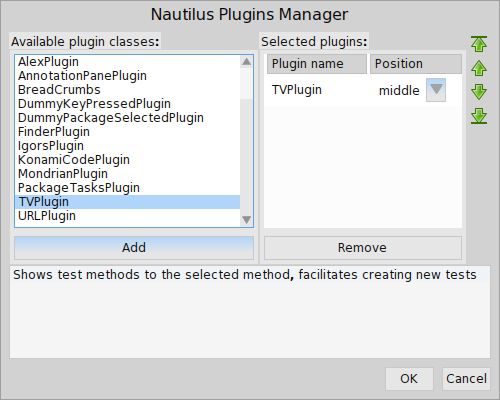
\includegraphics[scale=0.4]{screenshots/pluginManager.png}
        \captionof{figure}{The Nautilus Plugin Manager}
    }

		\item
		When you open a Nautilus\brs{what's a nautilus?} window from now on the plugin will be started until you remove it again using the Nautilus Plugins Manager. To verify if the plugin is activated check if this row is displayed in the position you selected.

		\parbox{\linewidth}{\centering
        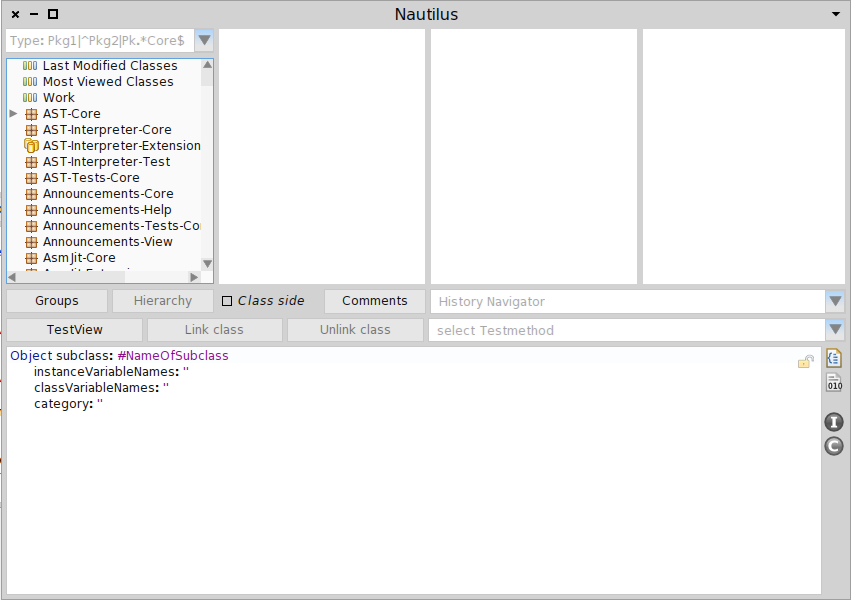
\includegraphics[scale=0.5]{screenshots/activatedPlugin.png}
        \captionof{figure}{TestView Plugin once it is active}
    }

	\end{enumerate}

\subsection{Adding a new test inside a new test class}
	\label{subsec:Creating a new test inside a new test class}
So now that the plugin is set up after following the steps in \autoref{subsec:Installation and activation} let us add a new test to a method. It is assumed here that you already have a method to test named ``doSomething'' inside of a class named ``MyClass'' and a package called ``MyPackage''.
	
\begin{enumerate}
\item Turn the TVPlugin on by clicking on the ``TestView'' button. Once this is done a second code panel will appear besides the code panel that shows the method do something.

		\parbox{\linewidth}{\centering
        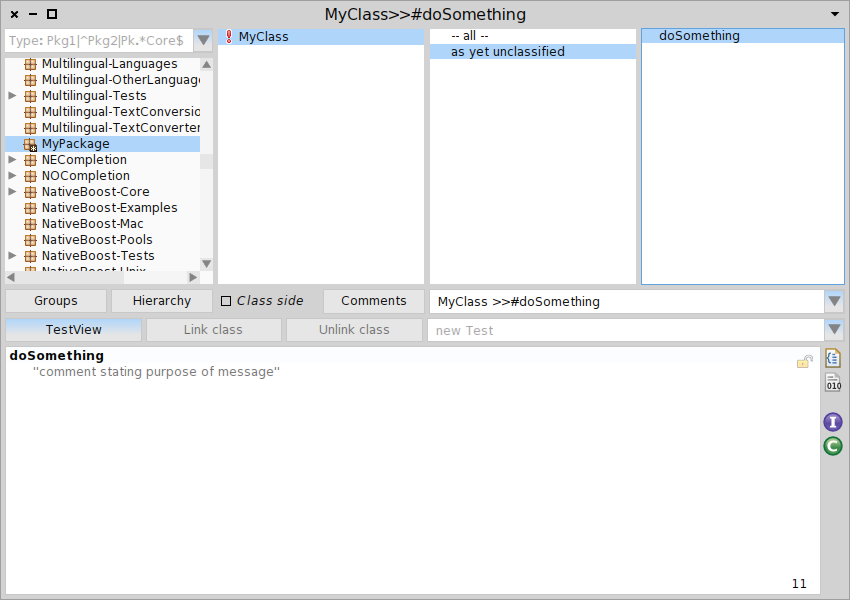
\includegraphics[scale=0.4]{screenshots/toggleButton.png}
        \captionof{figure}{Toggle the TVPlugin on}
        \label{fig:toggleButton}
    }
    
\item Make sure that you have selected the method for which you want to add a test in the Nautilus window. In this example this will be ``doSomething''.

\item Now open the dropList showing all the tests that have been found for ``doSomething''. In this case no tests will be found so only ``new Test'' will be selectable. Click on ``new Test''. By doing this you signal to the plugin that you want to add a test in a new test class.

		\parbox{\linewidth}{\centering
        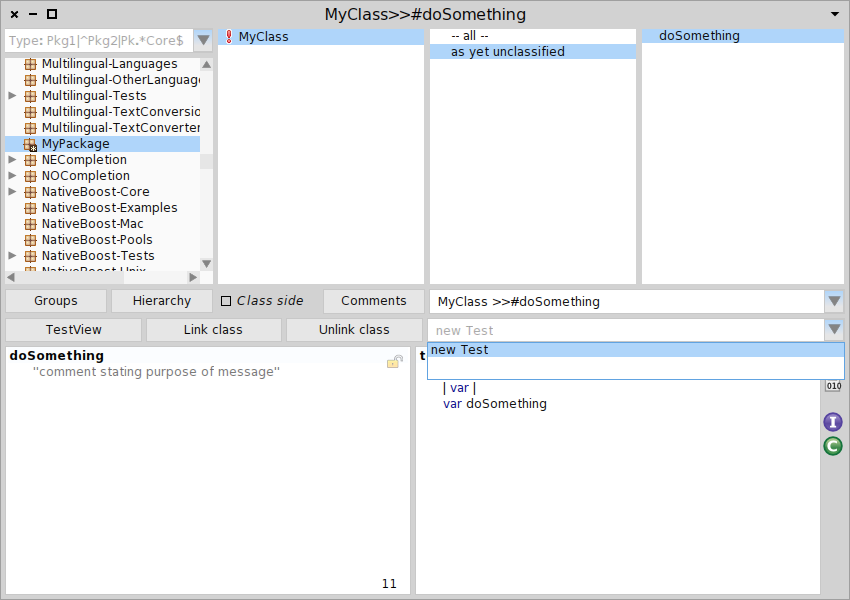
\includegraphics[scale=0.4]{screenshots/dropListNewTest.png}
        \captionof{figure}{Signal that you want to save the test in a new test class}
    }

\item Write your test in the right code panel. A template to start writing is already provided there by the TVPlugin.

\item Make sure the right code panel is still selected by clicking on it and accept your new test by pressing ctrl+s.

\item Since you previously selected ``new Test'' from the droplist the plugin is not sure in which test class this new test should be saved and will ask for clarification. A default name will already be in there but you can write your own test class name. Click ``OK'' when you have entered the name.
 
		\parbox{\linewidth}{\centering
        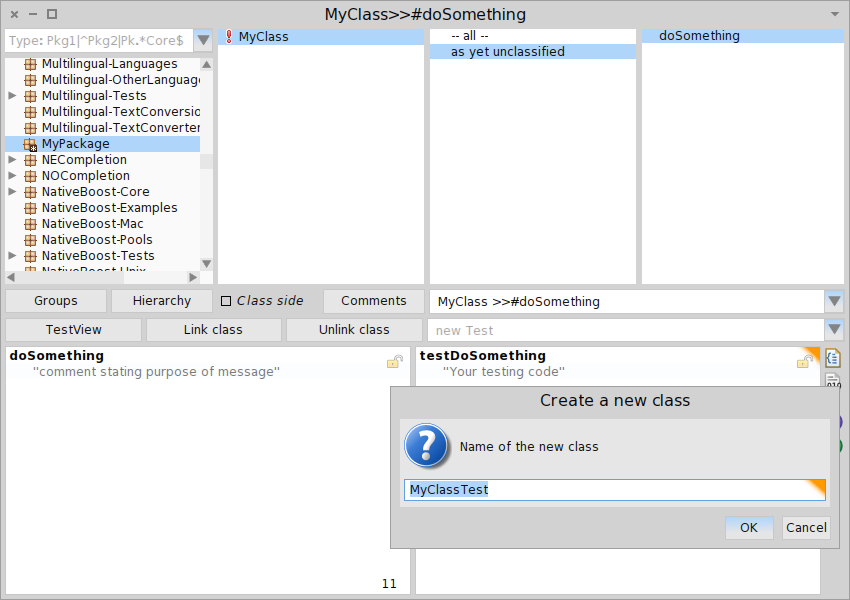
\includegraphics[scale=0.4]{screenshots/nameTestClass.png}
        \captionof{figure}{Name the new test class}
	}
        
\item Now you need to name in which package this new test class will be added. Similarly as before a default name will be provided but you can enter your own. Click ``OK'' to confirm the package name. This test package will now be created if it did not exist previously.

  	\parbox{\linewidth}{\centering
        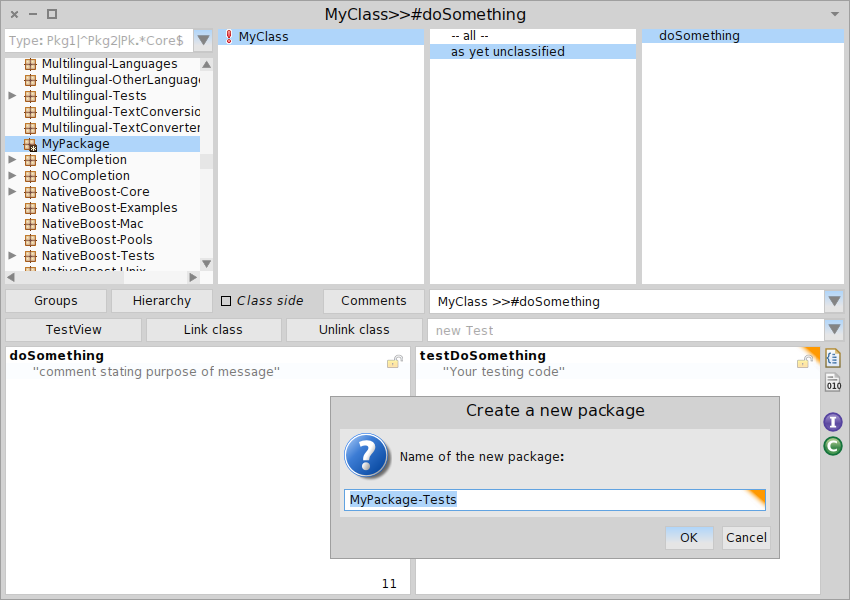
\includegraphics[scale=0.4]{screenshots/nameTestPackage.png}
        \captionof{figure}{Name the new test Package} 
	}
	
\item After the last step you can one last time change your mind and cancel the creation of the new class or enter new class and package names. Once you have finished checking an if necessary making additional changes click on ``OK''. The new test will now be added to the newly created test class and test package.

	\parbox{\linewidth}{\centering
        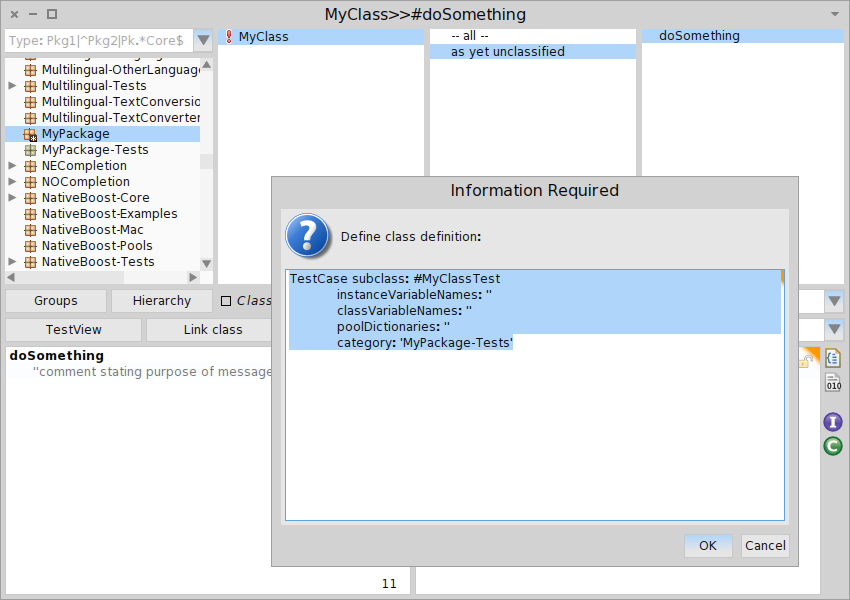
\includegraphics[scale=0.4]{screenshots/confirmNaming.png}
        \captionof{figure}{Confirm the new test class} 
	}

\end{enumerate}

\subsection{Adding a new to an existing test class}
	\label{subsec:Adding a new to an existing test class}
	In this section we will take a look at how to add a new test to an existing class. It is assumed that the plugin is activated. To do this you have to follow the steps outlined in \autoref{subsec:Installation and activation}.
	
\begin{enumerate}
	\item First make sure that the plugin is toggled on. If it is the Nautilus window has two code panels in the bottom. If it is not activate it by clicking the ``TestView'' button. See \autoref{fig:toggleButton} on how to toggle the plugin on.
	
	\item Make sure that you have selected the method for which you want to add a test in the Nautilus window. In this example this will be ``doSomething''.
	
	\item Now expand the droplist with the results and select any test that is contained in the class where you want your new test to be. In our case this is the ``MyClassTest'' so we select ``MyClassTest $>>$\#testDoSomething''.
	
	\parbox{\linewidth}{\centering
        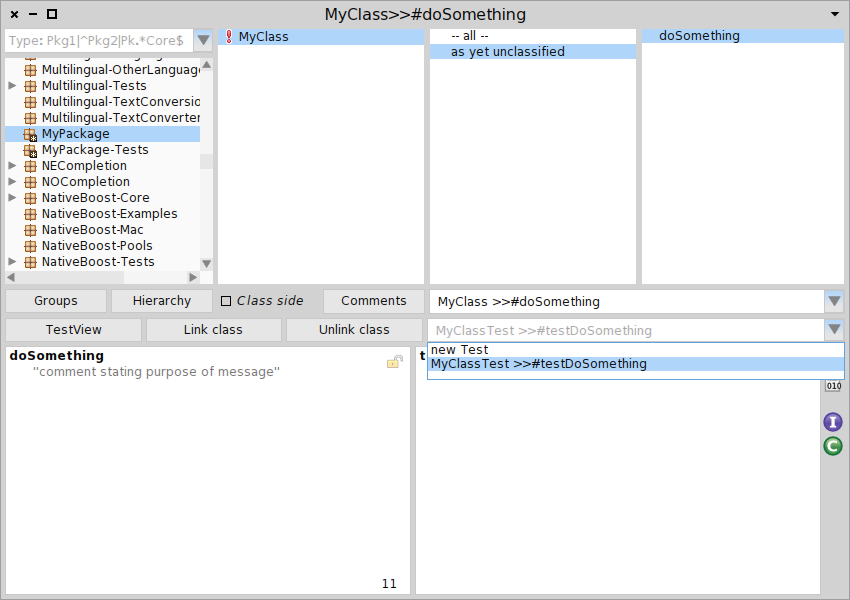
\includegraphics[scale=0.4]{screenshots/dropListExistingTestClass.png}
        \captionof{figure}{Select any test in the desired test class} 
	}
	
	\item The test you selected will now appear in the right code panel. Just write your test over it but make sure to give it a different name or else the test you selected will be overwritten. In our case we chose to name the new test method ``testDoSomethingElse''.
	
	\item Make sure the right code panel is still selected by clicking on it and accept your new test by pressing ctrl+s.
	
	\item Now your new test will be added to the test class you selected previously. You can verify this by opening the found tests droplist again and checking if your new test is there.
	
	\parbox{\linewidth}{\centering
        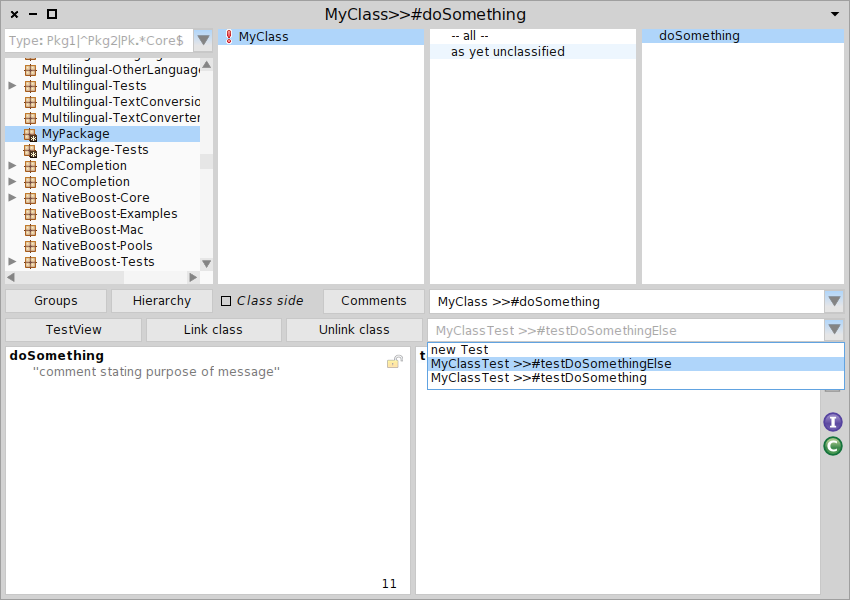
\includegraphics[scale=0.4]{screenshots/VerifyNewTestIsThere.png}
        \captionof{figure}{Check if your new test is shown here} 
	}	
\end{enumerate}

\subsection{Linking an existing test class}
	\label{subsec:Linking an existing test class}
When the TVPlugin does not find tests that you have created then this might be because it does not recognize the your test class as a possible source for tests to the class of the method that you currently have selected in the Nautilus class hierarchy. Here you find a step by step list of how to add your test class to the considered test classes.

\begin{enumerate}
	\item First in the Nautilus class hierarchy select the method that is missing tests in the found tests droplist.
	
	\item Click the ``Link class' ' button.
	
	\parbox{\linewidth}{\centering
        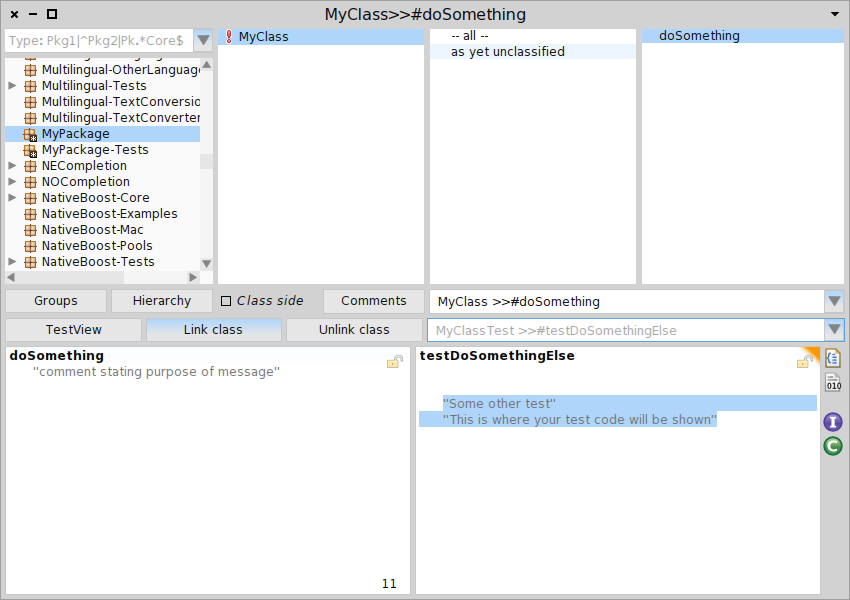
\includegraphics[scale=0.4]{screenshots/linkClassButton.png}
        \captionof{figure}{The ``Link class'' button} 
	}
	
	\item The TVPlugin will now ask which class you want to link as a test class to the class that is currently selected in the Nautilus class hierarchy. Enter the name of the desired test class and click ``OK''.
	
	\parbox{\linewidth}{\centering
        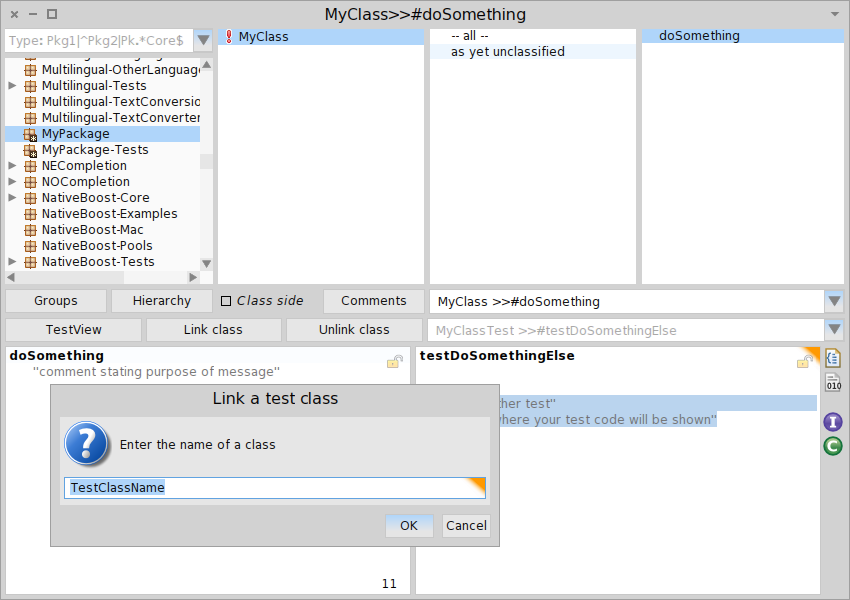
\includegraphics[scale=0.4]{screenshots/linkClassName.png}
        \captionof{figure}{Pop-up asking for the test class name} 
	}
	
	\item The specified test class is now added to the test classes that will be considered when searching for tests for the currently selected class. You can verify if it now works by opening the found tests dropview.

\end{enumerate}
	
\subsection{Unlinking an existing test class}
	\label{subsec:Unlinking an existing test class}
In case the TVPlugin shows you tests from a test class that you do not recognize as a test class for the currently selected class you can remove this class from consideration by using the ``Unlink class'' button.

\begin{enumerate}
	\item First in the Nautilus class hierarchy select the method that does show too many tests in the found tests droplist.
	
	\item Click the ``Unlink class' ' button.
	
	\parbox{\linewidth}{\centering
        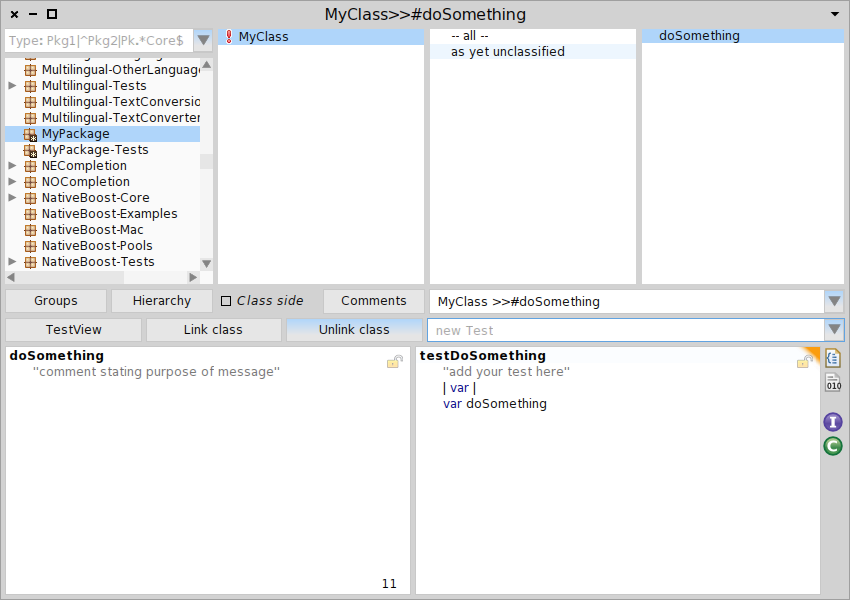
\includegraphics[scale=0.4]{screenshots/unlinkClassButton.png}
        \captionof{figure}{The ``Unlink class'' button} 
	}
	
	\item The TVPlugin will now ask which class you want to unlink as a test class to the class that is currently selected in the Nautilus class hierarchy. Enter the name of the desired test class and click ``OK''.
	
	\parbox{\linewidth}{\centering
        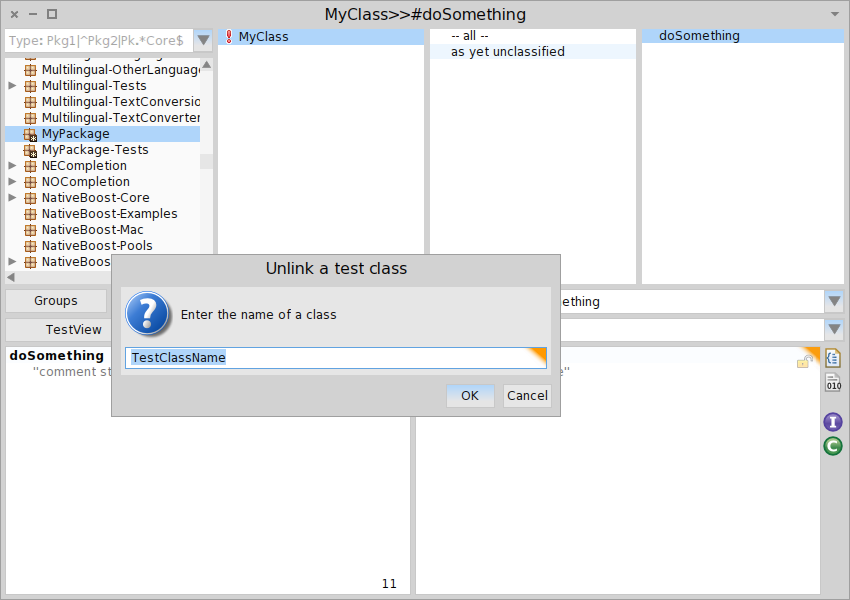
\includegraphics[scale=0.4]{screenshots/unlinkClassName.png}
        \captionof{figure}{Pop-up asking for the test class name} 
	}
	
	\item The specified test class is now removed from consideration. All test contained in this class will not be considered to be tests to the currently selected class. You can verify if this now works by opening the found tests dropview. No test contained in the unlinked class should be shown there.

\end{enumerate}

\subsection{Troubleshooting}
	\label{subsec:Troubleshooting}
	
	In this section some possible problems with the TVPlugin are listed and possible solutions to them outlined.

	\subsubsection{Tests are not found by the TVPlugin}
		\label{subsubsec:Tests are not found by the TVPlugin}
\meta{tests are missing in the found tests droplist}
	\meta{link your desired tests class}
	\meta{if this does not work your tests do not conform to the criteria, change them}
In case all tests from one or multiple tests classes are missing in the found test droplist you can add those test classes manually. If you want to add individual tests from a test class where already some tests are found then continue with \autoref{subsubsec:Add and remove individual tests from the corresponding test list to the selected method}. 

First make sure that your test classes are subclasses of "TestCase". If they are not the plugin will not consider them to be test classes. Simply go to the definition of your test classes and change the first line to "[YourClassName] subclass: \#TestCase". Check again if now the tests you from your test classes now are found.

If this does not help you can force the plugin to recognize your classes as test classes by linking the missing test classes to the currently selected class in the Nautilus class hierarchy. To do this follow the steps in \autoref{subsec:Linking an existing test class}. Recheck if your tests are found. If this does not work either then your tests themselves are written in a way that the TVPlugin does not recognize. You will have to change them so that they fulfill certain criteria. In this case also continue with \autoref{subsubsec:Add and remove individual tests from the corresponding test list to the selected method}.

\subsubsection{Tests that do not test the currently selected method are shown}
		\label{subsubsec:Tests that do not test the currently selected method are shown}
If the classes that contains these wrongly indentified tests do not contain any tests for the currently selected class then you can simply unlink these classes. Follow the steps outlined in \autoref{subsec:Unlinking an existing test class}. All the tests from these classes should new be gone from the found tests droplist.

If you want to remove only some tests from the found tests droplist then continue with \autoref{subsubsec:Add and remove individual tests from the corresponding test list to the selected method}. 

\subsubsection{Adding and removing individual tests to the tests found by the TVPlugin}
		\label{subsubsec:Add and remove individual tests from the corresponding test list to the selected method}
Both adding and removing an indiviual test from the tests that the TVPlugin finds are not a features that are directly supported. It is still possible to make these adjustments although likely not for all projects and not without changing your tests. The way the TVPlugin identifies individual tests as corresponding to the selected method has two components. The first one is soley based on the name of your test and the name of the method that it is supposed to test. The second one is if the test calls a method with the same name as the method that it supposedly tests.

\meta{naming criterion explained}
The name based criterion is a check if your test contains the full name of your method under test with at least one additonal time the substring "test". Examples of what is recognized as a test and what not based on this criterion are shown in \autoref{tab:name criterion examples}. This check is not case sensitive. And ":" from methods names with parameters will be ignored when looking for a test.

\begin{table}[h]
   \begin{tabular}{| c | c | c |}
     \hline
     \emph{Original method name} & \emph{Test names} & \emph{Not test names} \\ \hline
     doStuff & doStuffTest, testDoStuff, TestdosTuff & doStuff, doTestStuff, testStuff \\ 
     do:on: & testDoOn, testDoOn2, doOnTest & testDo:On:, do:testOn: \\ \hline
   \end{tabular} 
\end{table} 
\captionof{table}{Test naming criterion} 
\label{tab:name criterion examples}

\meta{cotains method selector the of the original method criterion}
The second criterion is if a method call is done inside of the possible test method to a method with the same name as the in the Nautils class hierachy selected method. This time the ":" are not removed from the check. If the supposed test method to a method named "do:on:" does call "doOn" then it will still not count as a test.

\meta{fulfill any criterion to add test to the testlist, break both to remove it from the list}
A test is recognized as such if either or both of these criteria are fulfilled. Conversely if neither is then the test is not considered a test to the selected method.
Adding a specific method to the tests found for a certain method can thus be done in two ways. Either make the name of the test contain the full name of the method in addition to "test" or call the method you want to test directly in the test. To remove a method from the found tests you have to make sure that the test name does not contain "test" and the full method name, and that inside of the test never a method with the same name as the supposed method under test is called. 
	
\begin{comment}
%%%%%%%%%%%%%%%%%%%%%%%%%%%%%%%%%%%%%%5
\section{Basic Components}
	\label{sec:Basic Components}
\brs{if you are talking about GUI components say so in section title, components can be anything}Here is a quick overview of all the visual elements can be found\brs{passive again}. The TVPlugin adds 3 buttons and one droplist to your Nautilus windows. The "TestView" button toggles the search for test methods to the currently selected method. If it is toggled on a second source code editor will appear at the bottom where the test methods will be displayed.\brs{pic, or did not happen} This list will change whenever a new method is selected in the Nautilus window.
The initial list shown in the droplist\brs{the what?} is composed of tests found through the search algorithm described under \ref{sec:The search Algorithm} \nameref{sec:The search Algorithm}\brs{use autoref in stead of ref and nameref}. The additional buttons "Link Class" and "Unlink Class" allow to customize this list if the search for any reason did not find some tests.

\section{The search Algorithm}
	\label{sec:The search Algorithm}
In this section I will provide a detailed explanation how corresponding tests to a certain method are found. It is a hierarchical search with two stages. \\ \par
\ugh{In the first stage all test classes are determined}\brs{what does this even mean?}. \ugh{For this all classes in the your environment are taken into consideration in the beginning. By the end of the first stage only those classes that inherit from "TestCase" as well as pass a substring search \brs{the what now?} in the class name are then passed over to the next step.} The substring search requires the name of the class in question to contain both "test" and the name of the selected class.\brs{oh... well, say this up front, don't make me guess what you mean by sub-string search}  If those two conditions are met then the class in question \ugh{is} \brs{is it really? how can you be so sure? if you are not 100\% sure, you need to say ``We consider it'' or something similar. } a test class of the selected class. The substring search is not case sensitive and the matches for "test" as well as the selected method can't overlap, meaning one letter can only be used to match partially either "test" or the selected class name.\brs{split the two conditions in two separate subsections or paragraphs and explain them in detail with either code, block diagram algorithms, math or something to help the reader understand}\\ \par

\begin{center}
   \begin{tabular}{| l | c | r |}
     \hline
     Original class name & Possible class names & Not a test class name \\ \hline
     String & StringTest, stringtest, TestString & String, Test, StrinTgEST \\ \hline
     Protest & ProtestTest & Protest \\

     \hline
   \end{tabular}
\end{center}
\todo{number this}
\brs{All tables, figures, listings, etc. MUST be numbered, named, and mentioned + refereed to in the text.}


In the second stage all test methods corresponding to the selected method out of all methods of the test classes are \ugh{determined} \brs{determining is not the right term for this, at least not in this phrasing. }. Similarly as before the test method name needs to contain the name of the selected method in addition to "test". \ugh{The second criterion is if the method in question uses the selector of the selected method.} \brs{you have like 4 or 5 different steps in this process and they are all divided in to pairs for some reason and all of them are 'in the second part, the second criteria etc. very confusing} Unlike stage one this stage\brs{name the stages, this usually helps} is fairly inclusive in that if only one of those criteria is satisfied it still qualifies as a test to the selected method.\\ \par
The two criteria of the second stage also serve to order the found test methods. The ones displayed on top satisfy both criteria. The ones that only satisfy the naming requirement are shown below these and the last ones are those that only contain the selector of the selected method. 

\section{Creating new Tests}
	\label{sec:Creating new Tests}
%move this to userGuide(partialy)
The other main functionality of the plugin besides finding tests is to facilitate creating them. When you have a method open in the first code editor to which you would like to add a test select the "new Test" option from the droplist\brs{run on sentence}. This option is an exception to the order described at the end of \ref{sec:The search Algorithm} \nameref{sec:The search Algorithm} and is always shown on top of the list. This option also can be found there regardless whether there were any tests found for the selected method. A template will appear in the second editor where the user can write the new test. When the test is accepted the user will be asked to name the class in which this test will be added. If the specified class doesn't exist it will be created and the user will be asked for a package to place it in. \\ \par 
A faster way to create a new test is to select an existing test from the droplist and alter it. By selecting a new name the old test will not be overwritten and the new test will be added to the class of the old test. Any test that was written using the second editor will result in its class being linked to the class of the selected method. This makes sure that the class in which the test was added is later recognized by the search algorithm even if its name does not confirm to the naming conventions of a test class.

\begin{figure}[h!]
	\centering
	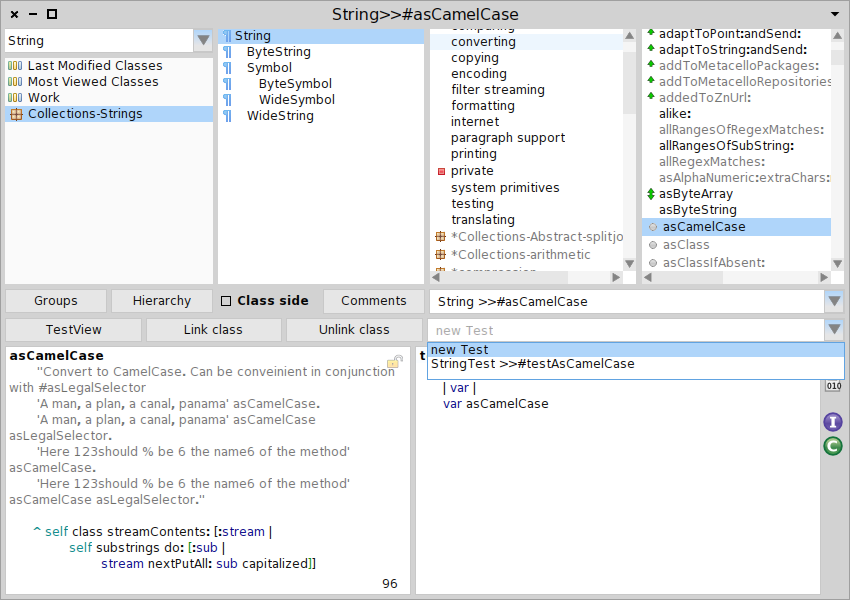
\includegraphics[scale=0.4]{screenshots/dropListOpen.png}
	\caption{Here the tests are selected}
\end{figure}

\chapter{User Guide}
	\label{cha:User Guide}
\end{comment}

%END Doc
%-------------------------------------------------------

%ideas: lack of large scale test suit support in TV(allan page beatiful testing), creating methods and classes from tests to better support tdd, better tdd support in general, unit testing cant be condensed to these core functionalities(e.g. test result collection and displaying is equaly as important), pctures for Pharo in related work chapter, test search only works method->tests not test->method

\bibliography{scg,thesis}
	\bibliographystyle{plain}
	
\end{document}
